\documentclass[a4wide]{scrartcl}

\usepackage{a4wide}
\usepackage[top=70pt,bottom=70pt,left=45pt,right=45pt]{geometry}
%\usepackage[margin=60pt]{geometry}
%Sonstiges
\usepackage{nameref}
\makeatletter
\newcommand*{\currentname}{\@currentlabelname}
\makeatother
\usepackage{graphicx}
\usepackage{nameref}

%Header
\usepackage[automark,headsepline]{scrpage2}
\pagestyle{scrheadings}
\ihead{GSoC 2018 - Faster Matrix Algebra for ATLAS}
\chead{}
\ohead{\currentname}
\ifoot{}
\cfoot{\thepage}
\ofoot{}

% References
\usepackage{hyperref}

%Language specific packages
%\usepackage[
%  left=1cm,
%  right=1cm,
%  top=1cm,
%  bottom=1cm,
%  includeheadfoot
%]{geometry}
\usepackage[utf8]{inputenc}
\usepackage[english]{babel}

%Listings
\usepackage{listings}
\usepackage{color}
\definecolor{codegreen}{RGB}{0,128,0}
\definecolor{codegray}{rgb}{0.5,0.5,0.5}
\definecolor{codepurple}{RGB}{175,0,219}
\definecolor{backcolour}{RGB}{241,241,241}
\definecolor{codestring}{RGB}{163,21,21}

\lstdefinestyle{mystyle}{
    language=c++,
    backgroundcolor=\color{backcolour},
    commentstyle=\color{codegreen},
    keywordstyle=\color{codepurple},
    numberstyle=\tiny\color{codegray},
    stringstyle=\color{codestring},
    basicstyle=\footnotesize,
    breakatwhitespace=false,
    breaklines=true,
    captionpos=b,
    keepspaces=true,
    numbers=left,
    numbersep=5pt,
    showspaces=false,
    showstringspaces=false,
    showtabs=false,
    tabsize=2,
}

\lstset{style=mystyle}
%amsPackages
\usepackage{amsmath}
\usepackage{amssymb}

\begin{document}
\title{Google Summer of Code 2018 - Faster Matrix Algebra for ATLAS}
\subtitle{Evaluation Test}
\author{\href{mailto: tellenbach@cip.ifi.lmu.de}{David A. Tellenbach}}
\maketitle
\section{Overview}
This documents gives an overview on my implementation of the evaluation test for the Google Summer of Code 2018 project \href{https://github.com/StewMH/GSoC2018/blob/master/evaluation_test.pdf}{Faster Matrix Algebra for ATLAS}. It discusses the current implementation of the class template \texttt{SymmetricMatrix<T, N>} and ideas how symmetric matrices could be added to the existing design of Eigen.
\section{Class Design}
The class \texttt{SymmetricMatrix} is actually a class template with two template parameters \texttt{typename Scalar} and \texttt{int Dimension}. The first describes the type of the values of the matrix, the second one its dimension. Since any symmetric matrix is a square matrix specifying one dimension is enough.
\subsection{Storage}
One of the tasks of this evaluation tests was to store only those elements of a symmetric matrix that determines it completely. A $(n \times n)$ matrix contains of $n^2$ elements. In the symmetric case the $ij$-th element is equal to the $ji$-th one, therefore it is sufficient to store
\[
\frac{n(n+1)}{2}    
\]
of its elements, e.g., the upper triangular part of it. Even though matrices are usually considered to be two-dimensional objects hardware memory is linear. The current implementation of the \texttt{SymmetricMatrix} class stores the matrix elements in either an \texttt{std::vector} or \texttt{std::array}. When storing these elements two storage orders can be considered: Row and column major storing.
\begin{description}
    \item[Row Major] The matrix elements are stored packed row by row as illustrated in \autoref{fig1}.
    \begin{figure}
    \centering
        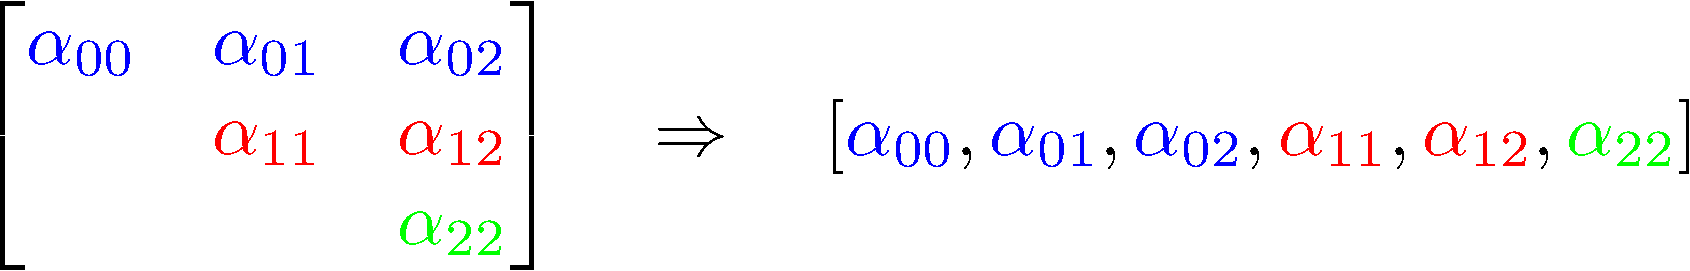
\includegraphics[scale=0.35]{img/RowMajor.pdf}
        \caption{Packed storage of a $3 \times 3$ matrix in row major order.}
        \label{fig1}
    \end{figure}
    Currently the SymmetricMatrix class stores matrix elements row major.
    \item[Column Major] The other storage order that can be considered is to store matrix elements packed column by column. Such a storage order is called column major and is illustrated in \autoref{fig2}.
    \begin{figure}
    \centering
        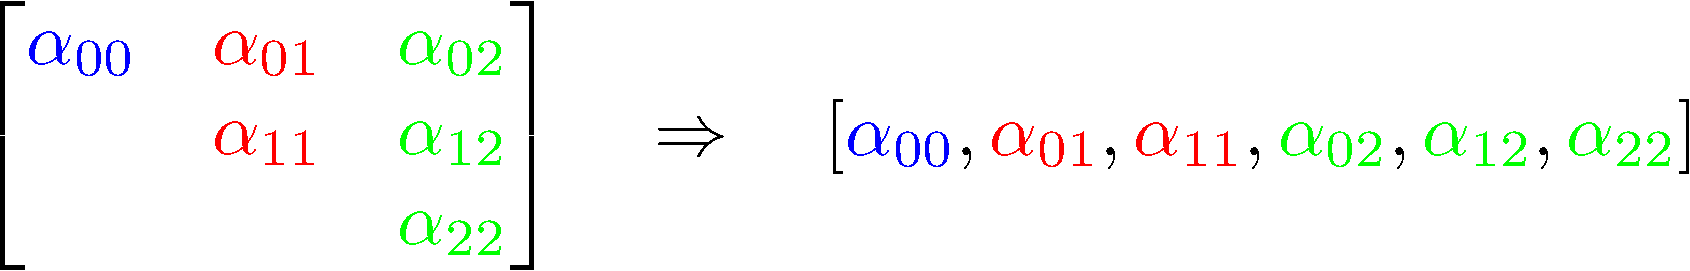
\includegraphics[scale=0.35]{img/ColumnMajor.pdf}
        \caption{Packed storage of a $3 \times 3$ matrix in column major order.}
        \label{fig2}
    \end{figure}
\end{description}
Storage order can dramatically determine the performance of matrix operations since it determines who matrix elements are loaded into cache. 
\subsection{Compile- and runtime}
Following the design of Eigen the implementation of this evaluation test contains both fixed and dynamically sized symmetric matrices. The generic class template \texttt{SymmetricMatrix<typename Scalar, int Dimension>} contains the implementation of fixed sized matrices. The elements are stored in an \texttt{std::array}. The size of this underlying container is calculated at compile-time. \newline
If the special dimension \texttt{Eigen::Dynamic} that is just a typedef for $-1$ is passed, the partial template specialization \texttt{SymmetricMatrix<typename Scalar, Eigen::Dynamic>} is used. This class is more flexible than the fixed sized case but is less performant as \autoref{tbl1} shows.\newline\newline
\begin{table}
\centering
\begin{tabular}{r|r|r}
Dimension & t1 (Fixed)  & t2 (Dynamic)  \\ \hline \hline
$10$  & $215$~ns & $731$~ns \\
$20$  & $656$~ns & $2306$~ns \\
$30$  & $1413$~ns & $4573$~ns \\
$40$  & $2530$~ns & $7844$~ns \\
$50$  & $3914$~ns & $11896$~ns \\
$60$  & $5812$~ns & $17107$~ns \\
$70$  & $7723$~ns & $23577$~ns \\
$80$  & $10185$~ns & $30322$~ns \\
$90$  & $13629$~ns & $39718$~ns \\
$100$ & $16239$~ns & $47402$~ns
\end{tabular}
\caption{Time consumption of adding fixed sized and dynamically sized matrices.}
\label{tbl1}
\end{table}
Since the memory allocation for fixed sized matrices is done during compilation it is completely located on the stack. Since stack size is limited matrices of this type are limited to relatively small dimensions. Large matrices containing thousands of elements should (and often must) be allocated on the heap. In this case dynamically sized matrices are the right choice.
\subsection{Addition and Subtraction}
Addition and subtraction are important component wise operations of matrices its complexity is always bounded from above by $n^2$ for a matrix of dimension $n$. Since we are not storing all $n^2$ elements of a symmetric matrix, we can perform even better.\newline
The actual implementation works just by adding up the elements of the underlying containers, i.e., instances of \texttt{std::array} in the fixed sized case and \texttt{std::vector} in the dynamically sized case. E.g., \autoref{lst1} show the implementation of the addition of two dynamically sized matrices.
\begin{table}
\begin{lstlisting}[caption={Overloaded operator $+$ for the addition of two dynamically sized matrices.},label=lst1]
SymmetricMatrix<Scalar>
operator+(const SymmetricMatrix<Scalar>& other) {
    // Check if both dynamic dimensions match
    if (dimension != other.dim()) {
        throw std::invalid_argument("Operation + cannot be performed "
                                    "for instances of SymmetricMatrix "
                                    "with not matching dimension");
        }

    // Construct new matrix and set underlying std::vector 
    // by passing the underlying std::vector of this
    SymmetricMatrix<Scalar> ret(elements);      

    // Just add up both underlying std::vector
    for (int i = 0; i < elements.size(); ++i) {
        ret.elements[i] += other.elements[i];
    }
    return ret;
}
\end{lstlisting}
\end{table}
\subsection{Multiplication}
Multiplication is a far more complex task than simple component wise operations like addition or subtraction. The simple implementation contains of three nested for-loops and the constant switch between matrix rows and matrix columns is pure cache horror. Big projects like BLAS have optimized matrix multiplication and its implementations like the Intel Math Kernel Library are complex and not easy to mimic. Trying to create an implementation beating or even being competitive with Eigen's internal multiplication implementation is no realistic task for this evaluation test.\newline
However the product of two symmetric matrices is in general not symmetric (it is and only is if the matrix product is commutative). Therefore this implementation uses the following trick: We construct instances of \texttt{Eigen::Matrix} from the symmetric matrices and use Eigen's internal mechanism to multiply these. Since the result of the multiplication will be \texttt{Eigen::Matrix} anyway, we won't have to issue about memory usage.\newline
One could now argue that the temporary constructed instances of \texttt{Eigen::Matrix} will consume memory. This is right in general but by using an optimization technique that can be avoided (at least when the compiler runs with optimizer flags). See \autoref{lst2} to see a concrete implementation of the multiplication of the symmetric matrices of dynamic size.
\begin{table}
\begin{lstlisting}[caption={Overloaded operator $*$ for the multiplication of two dynamically sized matrices.},label=lst2]
Eigen::Matrix<Scalar, Eigen::Dynamic, Eigen::Dynamic>
operator*(SymmetricMatrix<Scalar>& other) {
    // The instance of Eigen::Matrix is constructed in return statement
    // This allow the compiler to optimize temporary instances away
    return Eigen::Matrix<Scalar, Eigen::Dynamic, Eigen::Dynamic>(
               constructEigenMatrix() * other.constructEigenMatrix()
           );
}
\end{lstlisting}
\end{table}
\subsection{Runtime Exceptions and Compiletime Errors}
Another task of the evaluation test was to throw exceptions whenever an operations is performed where the dimensions of the operands don't match. In the particular case one has to consider the both cases of dynamically and fixed sized matrices differently:\newline
\begin{description}
\item[Fixed size operates with fixed size] The easiest case. The compiler performs statically type checks and the implementation guarantees that a compile time error will raise if the operands have non-matching dimensions. This holds for operations with fixed sized instances of SymmetricMatrix and fixed sized instances of \texttt{Eigen::Matrix}. See \autoref{lst3} for an example that will not compile.
\item[Fixed size operates with dynamic size] In these cases the implementation checks if the dimensions match during runtime. If they don't, an exception is thrown.
\item[Dynamic size operates with dynamic size] In these cases the implementation checks if the dimensions match during runtime. If they don't, an exception is thrown. See \autoref{lst4} for a try-catch example.
\end{description}
\begin{table}
\begin{lstlisting}[caption={Addition of matrices with different fixed size. This example will not compile.},label=lst3]
// Symmetric matrix of ints with fixed dimension 3 filled with random values
SymmetricMatrix<int, 3> mat1 = SymmetricMatrix<int, 3>::Random();

// Symmetric matrix of ints with fixed dimension 5 filled with random values
SymmetricMatrix<int, 5> mat2 = SymmetricMatrix<int, 5>::Random();

mat1 + mat2;    // Compiler error
\end{lstlisting}
\end{table}
\begin{table}
\begin{lstlisting}[caption={Addition of matrices with different dynamic size.},label=lst4]
// Symmetric matrix of ints with dynamic dimension 3 filled with random values
SymmetricMatrix<int> mat1 = SymmetricMatrix<int>::Random(3);

// Symmetric matrix of ints with dynamic dimension 5 filled with random values
SymmetricMatrix<int, 5> mat2 = SymmetricMatrix<int>::Random(5);

try {
    mat1 + mat2;
} catch (std::exception& ex) {
    std::cout << ex.what() << "\n";     
}
/* Output: Operation + cannot be performed for instances of SymmetricMatrix with not matching dimension */
\end{lstlisting}
\end{table}
\section{Benchmarks}
To measure the performance of the implementation of \texttt{SymmetricMatrix} the repository contains several benchmarks using the Google benchmark library. The following sections provide examples of these benchmarks run on my machine with the following hardware specifications:
\begin{description}
\item[Number of cores:]$8$
\item[Clock frequency per core:]$2.3~$GHz
\item[L1 Data cache size:]$32$~K ($4$x)
\item[L1 Instruction cache size:]$32$~K ($4$x)
\item[L2 Cache size:]$262$~K ($4$x)
\item[L3 Cache size:]$6291$~K ($1$x)
\end{description}

\subsection{add$\_$fixed.cc}
This benchmarks performs the addition of matrices of fixed size for dimensions from $10$ to $100$. \autoref{tbl2} shows the benchmark results.
\begin{table}
    \centering
\begin{tabular}{r|r|r|r}
    Dimension & t1 (Eigen + Eigen)  & t2 (Symmetric + Symmetric) & t3 (Symmetric + Eigen)  \\ \hline \hline
    $10$  & $8$~ns & $27$~ns & $107$~ns\\
    $20$  & $141$~ns & $52$~ns & $599$~ns\\
    $30$  & $101$~ns & $116$~ns & $978$~ns\\
    $40$  & $180$~ns & $194$~ns & $1826$~ns\\
    $50$  & $279$~ns & $253$~ns & $2566$~ns\\
    $60$  & $780$~ns & $523$~ns & $3704$~ns\\
    $70$  & $958$~ns & $749$~ns & $5049$~ns \\
    $80$  & $1211$~ns & $1144$~ns & $8532$~ns \\
    $90$  & $1488$~ns & $2024$~ns & $8460$~ns\\
    $100$ & $2024$~ns & $2594$~ns & $12782$~ns
    \end{tabular}
    \caption{Results of a run of benchmark add$\_$fixed.cc.}
    \label{tbl2}
\end{table}
While the addition of instances of \texttt{Eigen::Matrix} with instances of \texttt{Eigen::Matrix }is somehow comparable to the addition of instances of \texttt{SymmetricMatrix} with instances of \texttt{SymmetricMatrix} the addition of instances of \texttt{SymmetricMatrix} with instances of Eigen::Matrix is achieves a way lower performance. This is most likely an implementation issue and should definitely be improved.
\subsection{add$\_$dynamic.cc}
This benchmarks performs addition of dynamically sized matrices for dimensions from $1000$ to $10000$. \autoref{tbl3} provides benchmark results. While the addition of symmetric matrices with symmetric matrices can now even perform better that additions of arbitrary matrices with arbitrary matrices the addition of both perform bad again. However the results of the addition of two symmetric matrices is not satisfying even thought is performs as good as the addition of arbitrary matrices. Since way less elements are included a satisfying implementation would perform much better. 
\begin{table}
    \centering
\begin{tabular}{r|r|r|r}
    Dimension & t1 (Eigen + Eigen)  & t2 (Symmetric + Symmetric) & t3 (Symmetric + Eigen)  \\ \hline \hline
    $1000$  & $466$~us & $282$~us & $5910$~us\\
    $2000$  & $2343$~us & $3226$~us & $34419$~us\\
    $3000$  & $5687$~us & $8083$~us & $106047$~us\\
    $4000$  & $15054$~us & $14938$~us & $188352$~us\\
    $5000$  & $26146$~us & $26723$~us & $357040$~us\\
    $6000$  & $40217$~us & $37246$~us & $593490$~us\\
    $7000$  & $55773$~us & $59755$~us & $822445$~us \\
    $8000$  & $91013$~us & $77761$~us & $1097679$~us \\
    $9000$  & $110985$~us & $146855$~us & $1327157$~us\\
    $10000$ & $179361$~us & $191441$~us & $1925028$~us
    \end{tabular}
    \caption{Results of a run of benchmark add$\_$dynamic.cc.}
    \label{tbl3}
\end{table}
\subsection{mult$\_$fixed.cc}
This benchmarks performs the multiplication of matrices of fixed size for dimensions from $10$ to $100$. \autoref{tbl4} shows the benchmark results. In this case the multiplication of symmetric matrices with arbitrary ones performs better than the multiplication of symmetric with symmetric matrices. I think this is due to the fact the way multiplication is implemented by using the multiplication mechanism of Eigen. If one of the operands is an Eigen matrix, no construction of an instance of \texttt{Eigen::Matrix} from an instance of \texttt{SymmetricMatrix} has to be performed.\newline
However the performance of the matrix multiplication for all cases is way better than any naive implementation would be.
\begin{table}
    \centering
\begin{tabular}{r|r|r|r}
    Dimension & t1 (Eigen + Eigen)  & t2 (Symmetric + Symmetric) & t3 (Symmetric + Eigen)  \\ \hline \hline
    $10$  & $421$~ns & $850$~ns & $732$~ns\\
    $20$  & $1615$~ns & $2793$~ns & $2334$~ns\\
    $30$  & $4896$~ns & $7051$~ns & $6041$~ns\\
    $40$  & $10509$~ns & $14675$~ns & $12540$~ns\\
    $50$  & $20535$~ns & $25930$~ns & $23448$~ns\\
    $60$  & $34372$~ns & $41755$~ns & $39006$~ns\\
    $70$  & $54647$~ns & $64336$~ns & $59832$~ns \\
    $80$  & $82347$~ns & $96869$~ns & $91158$~ns \\
    $90$  & $114459$~ns & $129728$~ns & $122234$~ns\\
    $100$ & $154121$~ns & $178500$~ns & $170385$~ns
    \end{tabular}
    \caption{Results of a run of benchmark mult$\_$fixed.cc.}
    \label{tbl4}
\end{table}
\subsection{mult$\_$dynamic.cc}
The last benchmark performs multiplication of matrices with dynamic size. The results can be seen in \autoref{tbl5}. Now all three operation categories seem to be of comparable performance as \autoref{fig3} shows.
\begin{table}
    \centering
\begin{tabular}{r|r|r|r}
    Dimension & t1 (Eigen + Eigen)  & t2 (Symmetric + Symmetric) & t3 (Symmetric + Eigen)  \\ \hline \hline
    $1000$  & $149$~ms & $178$~ms & $161$~ms\\
    $2000$  & $1205$~ms & $1403$~ms & $1266$~ms\\
    $3000$  & $4049$~ms & $4612$~ms & $4315$~ms\\
    $4000$  & $9574$~ms & $11098$~ms & $10505$~ms\\
    $5000$  & $18632$~ms & $21189$~ms & $19754$~ms\\
    $6000$  & $34152$~ms & $35787$~ms & $33654$~ms\\
    $7000$  & $51049$~ms & $54553$~ms & $53570$~ms \\
    $8000$  & $76215$~ms & $81314$~ms & $80216$~ms \\
    $9000$  & $112280$~ms & $115698$~ms & $117566$~ms\\
    $10000$ & $160722$~ms & $158137$~ms & $156878$~ms
    \end{tabular}
    \caption{Results of a run of benchmark mult$\_$dynamic.cc.}
    \label{tbl5}
\end{table}
\begin{figure}
    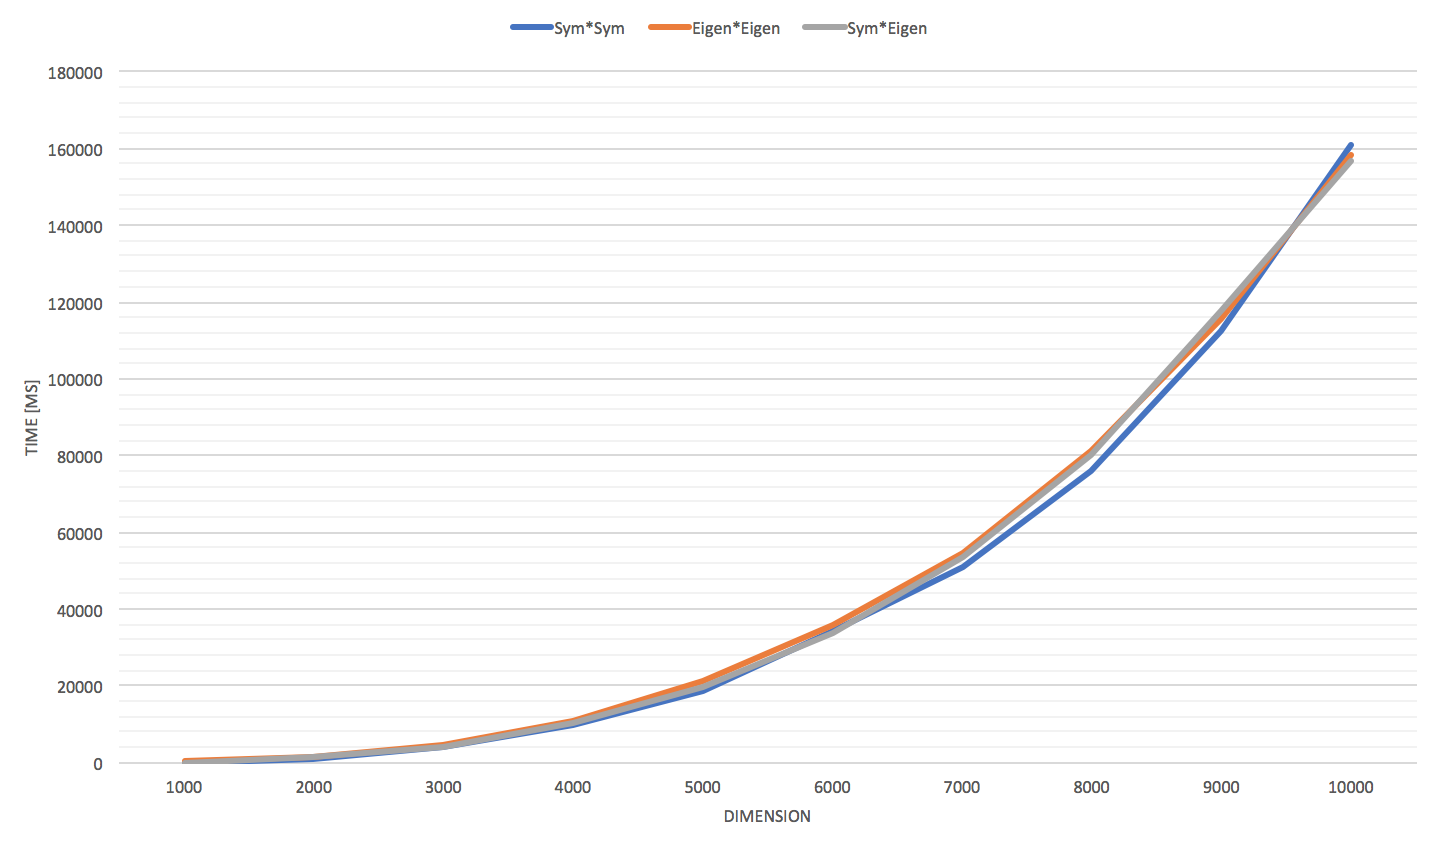
\includegraphics[width=\textwidth]{img/mult_dynamic.png}
    \caption{Graphical view on benchmark mutl$\_$dynamic.cc.}
    \label{fig3}
\end{figure}
\section{Future Work}
This section explains how I think an implementation of symmetric matrices could fit into the existing design of Eigen. Eigen provides effective and sophisticated mechanisms for the evaluation of matrix operations like a special form of lazy evaluation which is described here\footnote{\url{https://eigen.tuxfamily.org/dox/UserManual_UnderstandingEigen.html}} very well. A patch for Eigen should use these mechanisms which are of good performance and well tested. The next section gives an overview on the existing matrix classes in Eigen with the aim to get an idea how a new class could fit in.
\subsection{Existing matrix classes in Eigen}
Eigen provides mechanisms for handling different types of matrices. The following types are supported:
\begin{description}
\item[Dense matrices]Matrices were all elements are stored. Matrices of type Eigen::Matrix are dense.
\item[Sparse matrices]Sparse matrices, i.e., matrices were most of the elements are $0$. This class uses a special storage mechanism such that only the non-zero elements are stored together with information about their position in the matrix.
\item[Diagonal matrices]Diagonal matrices. The elements are stored in a simple container and no mechanism for determining their position in the matrix is needed. The position is clear from the position in the storing container.
\end{description}
Obviously the storage mechanism of dense matrices is not well suited for storing symmetric matrices. Neither is the mechanism of sparse matrices  good for us. We don't need a special mechanism to reconstruct the position of matrix elements. The idea of diagonal matrices seems to be exactly what we want: We just store matrix elements in a container and their position in the matrix is determined completely by their position in the container. \newline
Therefore the symmetric matrix class will be a sibling of the diagonal matrix class in Eigen's class hierarchy. The source for \texttt{Eigen::DiagonalMatrix} can be found here\footnote{\url{https://eigen.tuxfamily.org/dox/DiagonalMatrix_8h_source.html}}. As we can see it is basically derived from the class \texttt{Eigen::EigenBase}. \texttt{Eigen::EigenBase} is the base class for all matrices and appears to be the greatest common class in the class hierarchy of all matrix classes described above.
\subsection{Implementation ideas}
Following this idea my idea for an implementation of symmetric matrices in Eigen is to derive the class from \texttt{Eigen::EigenBase}. This allows using the high performant mechanisms that Eigen provides while defining a custom storage type.
\end{document}












